\chapter{Improving Readout Fidelity}
While considering the entire time-evolution dynamics can prove more insight in our system, it can also be used in different ways to optimize the system further. In this section, we will consider how to use the entire time-trace and knowledge of the dynamics to perform the best possible readout. In this section, we will consider the $I$ and $Q$ signal from either experiment or from simulation. In the experiment, $I$ and $Q$ comes from the stochastic trajectory process, while in experiment it is the demodulated signal from the IQ mixer.

\section{Readout Fidelity}
Before talking about, how we improve the readout, we need to discuss, what a good readout is. If doing a readout is achieving a scheme:

\begin{itemize}
    \item Given a state $\rho_{\text{true}}$ a readout predicts $\rho_{\text{pred}}$, such that $\rho_{\text{pred}}$ is on average as close to $\rho_{\text{true}}$ as possible.
\end{itemize}
Now the task is to define a quantity for "closeness" between a density matrix and our prediction. Mathematically, we can achieve this by defining a formal distance, such as the trace-norm on the vector space of $2\times2$ matrices: $\mathcal{M}^2$. \todo{Find source. Right now we use wikipedia...}
\begin{equation}
    ||\rho_{\text{pred}} - \rho_{\text{true}}|| = \Tr \left[\sqrt{\left(\rho_{\text{pred}} - \rho_{\text{true}} \right)^\dagger \left(\rho_{\text{pred}} - \rho_{\text{true}} \right)} \right]
\end{equation}
which has the desired properties like being $||\rho_{\text{pred}} - \rho_{\text{true}}|| = 0$, if our prediction is correct. To make this more familiar for a quantum physicist, we instead use the fidelity, which has a general form defined by:
\begin{equation}
    F(\sigma, \rho) = \left(\Tr\sqrt{\sqrt{\rho} \sigma \sqrt{\rho}}\right)^2
\end{equation}
which is related to the trace norm by inequalities\footnote{Write them here}, but also has nice properties, that it reduce significantly if one of the states are pure. In our schemes the readout will always predict pure state of either $\ket{1}\bra{1}$ or $\ket{0}\bra{0}$. In this case $\sigma = \ket{k}\bra{k}$ and the full equation can be written as:  \todo{Maybe add explanation of $\sqrt{\rho}$ and the equality of the swapped version.}
\begin{align*}
    F(\sigma, \rho) = F(\rho, \sigma) &= \left(\Tr\sqrt{\sqrt{\sigma} \rho \sqrt{\sigma}}\right)^2 \\
    &= \Big(\Tr \left(\ket{k}\mel{k}{\rho}{k}\bra{k}\right)\Big)^2\\
    &= \mel{k}{\rho}{k}
\end{align*}
Given the fidelity of one measurement is however hard, and we estimate this by repeating the comparison $n$-times. We also need to measure both $0$ and $1$, so we have to do a mean over this as well. This gives an expectation value of:
\begin{equation}
    \mathbf{E}\left[F(\sigma, \rho)\right] = \frac12 \sum_{k \in \{0, 1\}}\frac{1}{N}\sum_n^N F(\sigma, \rho)
\end{equation}
While this is a valid average, it gives us $\mathbf{E}(F_{\sigma, \rho}) = \frac12$ for a completely random classification\footnote{And a classification scheme with $F<\frac12$ can be better by just swapping the output labels}. Thus the expectation value is often rescaled, such that a random classification gives $0$:
\begin{equation}
    F_{\text{readout}} = 2 \mathbf{E}\left[F(\sigma, \rho)\right] - 1 = 2 ( \mathbf{E}F(0, \rho_0) + \mathbf{E}F(1, \rho_1) ) - 1 
\end{equation}
Which can be written in terms of the infidelities $F(0, \rho_0) = 1 - F(1, \rho_0)$:
\begin{equation}
    F_{\text{readout}} = 1 - \mathbf{E}F(0, \rho_1) - \mathbf{E}F(1, \rho_0)
\end{equation}
Which is the definition we will be using to define the "goodness" of a readout. \todo{This section is at the moment a bit sloppy.}

\section{Determining the Readout Fidelity}
Given a set of IQ measurement of the qubit initialized in $\ket{0}$ and $\ket{1}$ respectively\todo{Maybe describe experiment with a circuit}, we want to combine it to maximize the separation between the $\ket{0}$ and $\ket{1}$ state. If the resonator has reached its steady state and the measurements come from a Gaussian distribution, it is sufficient to sum/mean the whole trace, and compare the final distributions. Under this assumption we will get a distribution of IQ values. 

\begin{marginfigure}
    \centering
    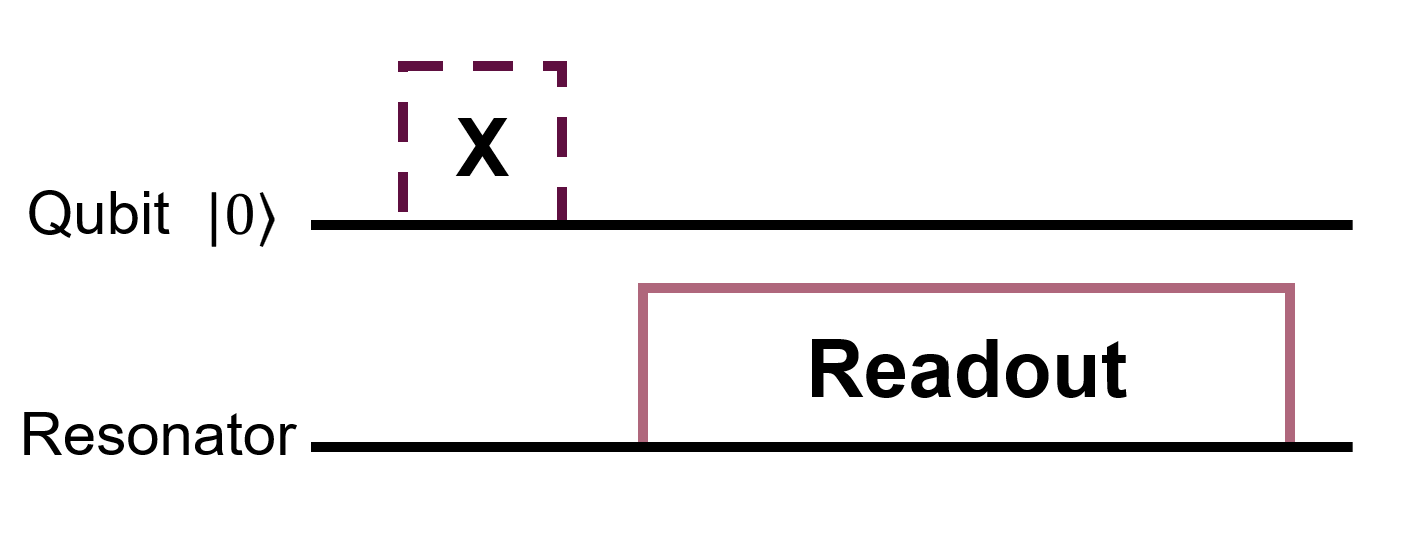
\includegraphics[]{Figs/circuits/readout_test.png}
    \caption{Circuit displaying the process of making a readout test. In half the initialization, an $X$ gate is applied to excite the qubit to $\ket{1}$. This is followed by a readout pulse on the resonator.}
    \label{fig:circuit_qubit_readout_test}
\end{marginfigure}

We now pick the projection line through this plane that best separates the $\ket{0}$ and $\ket{1}$ group. This can for example be done by using an LDA algorithm. On this axis, we can now set a threshold. If we set it such that the fidelity is maximized, we have defined our simple readout scheme. The process can be see in figure \ref{fig:simple_weights_fidelty}.

\begin{figure*}
    \centering
    \missingfigure{Illustration of readout process. Summation of signal }
    \caption{Caption}
    \label{fig:simple_weights_fidelty}
\end{figure*}

In this example the measurements was done on ??? samples. Giving readout fidelity ... \todo{Perform simple analysis of the weights. Probably do a table with some sub information.} 

\section{Filtering and Weights}
Just summing to get a good a classification works well if the points are steady state and stays there. In reality however, we might have different other attributes in the readout signal, that we want to weigh differently. A typical example, is that the qubit ramp-up interval will have less separation than in the steady state. Further, the qubit will also experiment energy decay from $\ket{1}\to \ket{0}$\footnote{Or absorp energy to go the other way}. Or we can also include data after we stopped driving, where the resonator stays will decay to the vacuum state, but again be closer.

\subsection{Weighting of the Input}
Under the assumption that the measured signal from the resonator will be Gaussian in the IQ plane, the points at different times are uncorrelated and symmetric \todo{cite Machine Learning for Discriminating Quantum Measurement Trajectories
and Improving Readout}  it is possible to derive the optimal linear weights. To see this, we allow for a weighting of each time step in each quadrature. Then the signal from equation \ref{fig:stochastic_signal_hetereodyne} takes the form is $\sum_{x = I, Q}\sum_t k_{x, t} \cdot x_t$. If we subtract the records when starting from the ground or exciting state, we will write the total separation signal as:\todo{How is this related to the approximations listed. T1 $\to$ gaussian is a stretch}
\begin{equation}
    \Delta S = \sum_X \sum_t k_{x, t} (\expval{X_0 - X_1} + \xi_t)
\end{equation}
Where we have collected the noise terms in some $\xi_t$. Then to maximize the SNR\todo{Define Signal to noise and relate it to fidelty above}, we find the mean and variance of the separated signal as:
\begin{equation}
    \SNR = \frac{|\expval{\Delta S}|^2}{\Var(\Delta S)} 
\end{equation}
where we can find the mean and variance of the signal as:
\begin{align}
    \expval{\Delta S} &= \sum_X \sum_t k_{x, t} (\expval{X_0 - X_1} \\
    \Var(\Delta S) &= \sum_X \sum_t k_{x, t}^2 \left( \Var(\expval{X_0 - X_1}) + \Var(\xi) \right)
\end{align}
Now maxizing the SNR by $\partial / \partial k_{x, t}$, we find that we should set:
\begin{equation}
    k_{x, t} = \frac{\expval{X_0 - X_1}}{\Var(\Delta S)}
\end{equation}
Where we will determine the variance and average expected difference experimentally by performing a set of measurement and calculating the mean difference and variance to determine the weights. \todo{cite Tomography via correlation of noisy measurement records}

In figure \ref{fig:matched_weights_fidelty} the experiment shown in figure \ref{fig:simple_weights_fidelty} is repeated but with calculated linear weights before rotating. As we can see the readout fidelty is now... \todo{Write this in}

\begin{figure*}
    \centering
    \missingfigure{Weights and improvement of the signal}
    \caption{Caption}
    \label{fig:matched_weights_fidelty}
\end{figure*}


\subsection{Non-Linear Classifications}
The classification scheme above is very common, since it can be combined with the demodulation (both linear operation) and is able to be run on the FPGA. This makes it very fast and easy to calibrate. However, the assumption are not entirely realistic. This becomes very clear, when we think about the effects of $T_1$ which splits ... \todo{Is $T_1$ a good example? What else do we violate}. One could setup allow for covariance between measurements or nonlinear kernels. Or a different method is to use Machine Learning methods to distinguish the trajectories. This allows for the possibility of weighting the inputs differently depending on the beginning of the signal beyond the average behaviour.\todo{Do we want to try this quick? Otherwise, we can reduce this to a comment in the above section.}



\section{Postselection}
In some instances, we do not mind running with a large overhead in order to increase our readout fidelity. In these cases, we can instead associate a probability of a given trajectory belonging to the $0$ or $1$ group and then pick those with the highest probabilities. Since $T_1$ decay tends to happen somewhere during the measurement, the points will often be placed in some tail going from $1 \to 0$. If we instead only keep the trajectories with the highest probability, we sacrifice all the points in the middle.

\begin{figure}
    \centering
    \missingfigure{Trading overhead. We want a logarithmic x-axis with the scaling of points}
    \caption{Caption}
    \label{fig:enter-label}
\end{figure}

Up to some point we get an improved fidelty. The maximum is however not $1$. This is credited to the state preparation errors since wrongly prepared qubits in $1$ will behave like $0$ and will not be distinguishable in any measurement. 


The following sections is also possible:
\begin{itemize}
    \item Adjusting Pulse Parameters
    \item Strategies
    \item Counter Depopulation Pulse
\end{itemize}

% \section{Adjusting Pulse Parameters*}
% \begin{itemize}
%     \item Reading out after, since we have to wait for depopulation anyways.
% \end{itemize}

% \section{Strategies*}
% \begin{itemize}
%     \item This can be kicking the qubit with a $\pi_{12}$ pulse. 
% \end{itemize}

% \section{Counter Depopulation Pulse*}
% \begin{itemize}
%     \item Stimulated depopulation
% \end{itemize}